\chapter{LOCALIZAÇÃO DAS MEDIDAS DE COMPRIMENTO E LARGURA}\label{ap:localizacao-medidas}

Este apêndice apresenta a localização dos segmentos utilizados na determinação do comprimento longitudinal máximo (Lₜ) e da largura transversal máxima (Wₑ) de cada depósito e evento. Nas representações, os segmentos de comprimento são indicados em preto e os segmentos de largura em branco. Os valores resultantes dessas medições são apresentados nas respectivas tabelas do capítulo de resultados.

\begin{figure}[htbp]
  \centering
  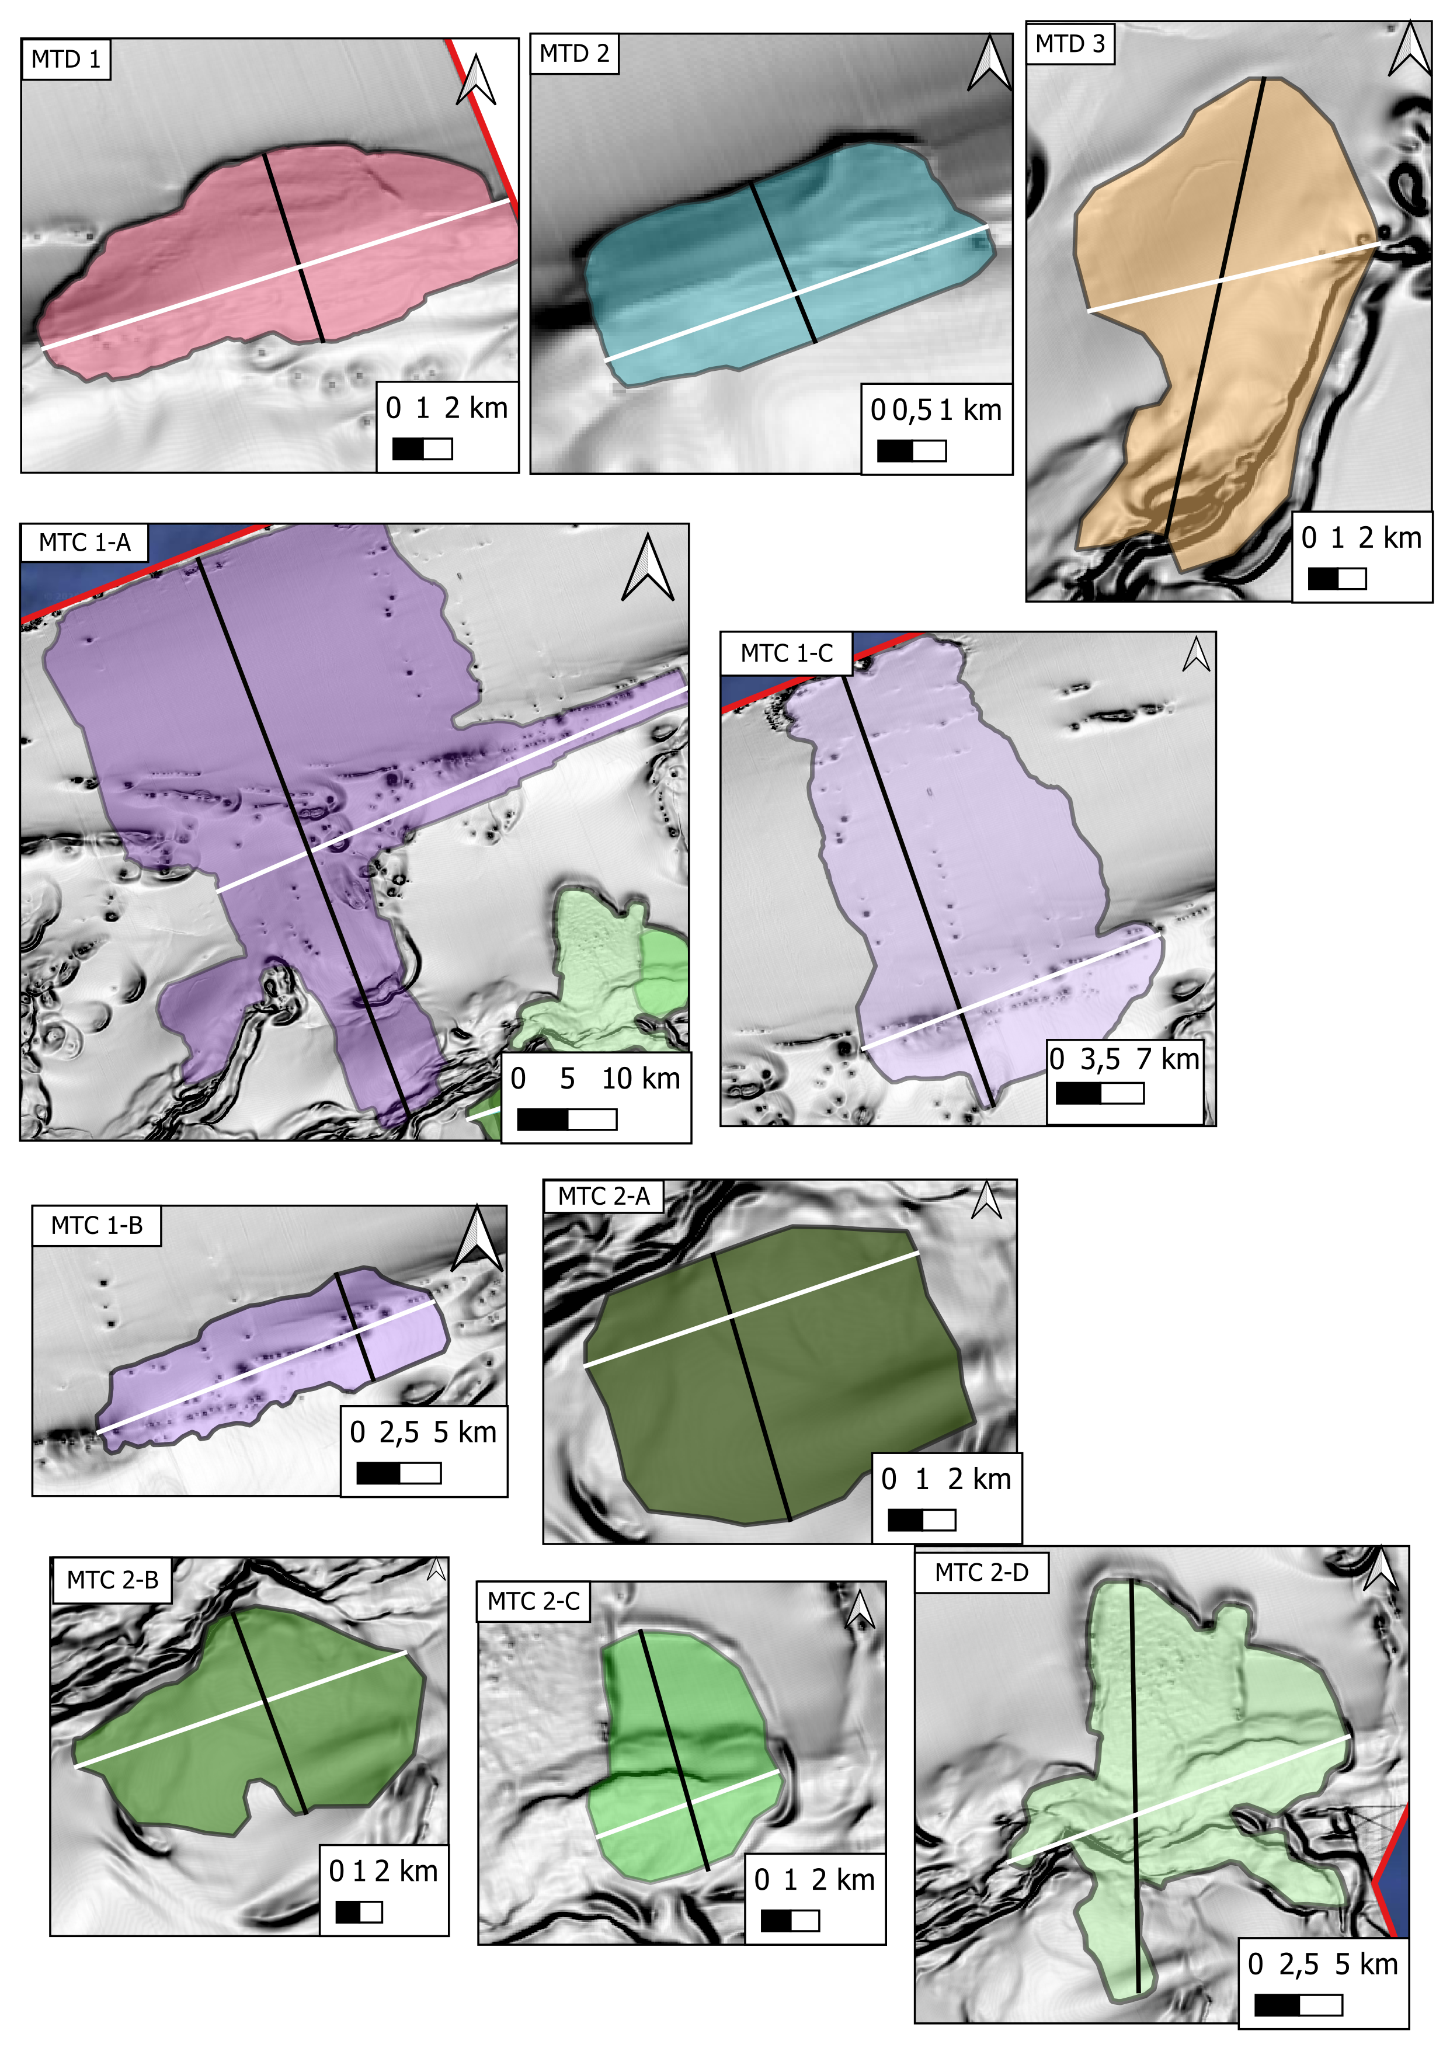
\includegraphics[width=\textwidth,height=0.80\textheight,keepaspectratio]{figuras/resultados/figura-B-1-localizacao-dos-segmentos-utilizados-nas-medicoe.png}
  \caption{Localização dos segmentos utilizados nas medições do comprimento longitudinal máximo (Lₜ), em preto, e da largura transversal máxima (Wₑ), em branco, para os depósitos e eventos analisados.}
  \label{fig:resultado-B-1}
\end{figure}
